OpenQuake computes probabilistic seismic hazard using two different methodologies: the classical one and a methodology based on stochastic event set generation.

The classical PSHA methodology implemented \citep{cornell1968,mcguire2004} follows the formulation presented by \citet{field2003}. This particular formulation has the distinctive property of performing the entire calculation using probabilities, as also originally proposed by \citet{chiang1984}, instead of working with occurrence rates like in most of the commonest PSHA codes \citep[see for instance][]{bender1987}. 
%
The OpenSHA methodology has also the clear advantage of decoupling the creation of the probabilistic seismicity occurrence model (in the OpenSHA terminology this is defined as the Earthquake Rupture Forecast) from the assumption of a Poissonian temporal occurrence model. 
%
By assuming that the contributions to hazard coming from multiple occurrences in a seismic source are negligible i.e. the probability that a source will generate two or more occurrences within the time span fixed for the analysis is equal to zero - as proposed by \citet{field2003} - the calculation of hazard following this methodology is completely consistent with the most classical procedure.
% 
\citet{pagani2007} proved that this assumption holds at least for some prototypal situations.

Two are the main steps composing the classical PSHA calculation procedure embedded in OpenSHA (and thus OpenQuake): the creation of the Earthquake Rupture Forecast and the calculation of the hazard at the site.
The creation of the Earthquake Rupture Forecast (i.e. the seismicity occurrence model) - corresponding to a list of all possible ruptures on each source incliuded in the model with associated probability of occurrence in a given time span - is a first step necessary also in the case of PSHA calculations based on a stochastic event set based methodology. The creation of the ERF is discussed in Chapter \ref{chap:erf} at page \pageref{chap:erf}.
%
The second phase in the classical PSHA approach correspons to the calculation of hazard at the site by combining the probabilistic seismicity occurrence model with a ground motion prediction equation (in the OpenSHA jargon also called Intensity Measure Relationship). It will be described in the following section (\ref{chap:classic_psha} at page \pageref{chap:classic_psha}).

The stochastic event based PSHA calculation procedure resembles recent approaches proposed in the literature (see for example \citet{musson2000} and references therein). The major advantages of this approach are that (1) hazard can be directly linked to a sequence of earthquakes and (2) the residuals of ground motion on each investigated site 
%
This methodology is more extensively described in section \ref{chap:stochastic_psha} at page \pageref{chap:stochastic_psha}.

%
%-------------------------------------------------------------------------------
\section{Classical PSHA calculator}
\label{chap:classic_psha}
%
In the simplest case, the classical PSHA calculation kernel takes as input: 
%
\begin{itemize}
%
\item An Earthquake Rupture Forecast (ERF - also called Probabilistic Seismicity Occurrence Model). An ERF is a list of all the possible ruptures occurring on all the seismic sources included in a Source Model. Each rupture $Rup$ is associated with a probability of occurrence $P(Rup|t)$ referred to the time span $t$ fixed for the analysis. 
%
\item A Ground Motion Prediction Equation (GMPE). A GMPE is an equation that - given some fundamental parameters characterizing the source, the propagation
path and the site (in the simplest case magnitude, distance and V$_\text{S,30}$) - computes the value $GM$ of a (scalar) parameter describing ground motion intensity. $gm$ is always accompanied by a standard deviation value $\sigma_{gm,T}$ specifying the aleatoric variability associated to $gm$.
\end{itemize}

We start the description of the classical PSHA procedure by illustrating the calculation of the probability of exceedance of a ground motion value $gm$ in a investigation time $t$ at site $site$ given a rupture $rup$ within source $source$; $rup$ is a rupture produced by one of the seismic sources included in the Earthquake Rupture Forecast. 
%
This probability corresponds to the product between the probability of occurrence of $rup$ in a time $t$ and the conditional probability of exceeding $gm$ at $site$ given the occurrence of $rup$. Analytically this corresponds to:
\begin{equation}
P_{site,source,rup}(GM \geq gm|t) = P(Rup_{source}|t)\,P_{site}(GM\geq gm|Rup_{source})
\label{eq:prob_gm_ex_one_rup}
\end{equation}
%
Some notes regarding the equation above:
\begin{itemize}
\item The probability of exceedance of a value of ground motion $gm$ at $site$ given a rupture (i.e. $P_{site}(GM\geq gm|Rup_{source})$) is computed (1) by assuming that the logarithm of ground motion is normally distributed. The mean - $\overline{log(gm)}$ - of this distribution is computed with a ground motion prediction equation and the standard deviation $\sigma$ is usually provided with the adopted GMPE.
\item The ground motion temporal occurrence is controlled by the manifestation of the rupture $rup$ during the investigation time $t$.  
\end{itemize}

%

%
If the source contains several ruptures that we assume mutually exclusive, the probability that at least one rupture will generate one exceedance corresponds to the difference between unity and the probability that none of the ruptures will generate an exceedence of $gm$:
\begin{equation}
P_{site,source}(GM\geq gm|t) = 1 - \sum_{}^{R} \Big( P(Rup|t)\,P_{site,source}(GM\geq gm|Rup) \Big)
\label{eq:class_psha_1}
\end{equation}
$R$ corresponds to the number of ruptures. We compute the final value of hazard at the site $site$ by considering the contributions from the sources whose ruptures collectively create the ERF:
%
\begin{equation}
P_{site}(GM \geq gm|t) = 1 - \prod_{}^{S} \Big( 1-P_{site,source}(GM\geq gm|Rup) \Big)
\label{eq:class_psha_2}
\end{equation}
%
$S$ corresponds to the number of seismic sources. Combining equations \ref{eq:class_psha_1} and \ref{eq:class_psha_2} we obtain \cite[][equation 4, page 410]{field2003}:
%
\begin{equation}
P_{site}(GM\geq gm)=1-\prod\limits_{}^{S} 
	\Big( 
		1-\sum_{}^{R} \Big( P(Rup|t)\,P_{site}(GM\geq gm|Rup)
	\Big)
\label{eq:PSHA_calculation}
\end{equation}

%  - - - - - - - - - - - - - - - - - - - - - - - - - - - - - - - - - - - - - - -
\subsection{Relaxing the assumption of a single rupture per source over the investigation time}
%
Let's start by considering equation A8 described in \citet{field2003}:
%
\begin{equation}
P_{site}(GM\geq gm)= 
	1-\prod\limits_{}^{S} 
	\left[\sum\limits_{s=0}^{+\infty}
	\left(P(S=s) 
	\left(
		1-\sum\limits_{j=0}^{j(i)}\sum\limits_{s=0}^{K(i,j)} 
		P(m_{i,j}) 
		P(R_{i,j,k}|m_{i,j}) P(U\geq u|m_{i,j},R_{i,j,k})
	\right)
	\right)^{s}
	\right] 
\end{equation}
where $l$ i the number of sources.

%  - - - - - - - - - - - - - - - - - - - - - - - - - - - - - - - - - - - - - - -
\subsection{Vector-valued PSHA (VPSHA)}
This is a procedure originally proposed by \citet{bazzurro2002}
%
% ==============================================================================
\clearpage\newpage
\section{Stochastic PSHA calculator}
\label{chap:stochastic_psha}
%
The calculation of stochastic event sets \index{Stochastic event set} and the corresponding ground motion fields is a methodology tightly connected with a specific seismic risk analysis of common use within the insurance and re-insurance industry (CITATION). 

OpenQuake, given a Source System, can generate a number of seismicity histories, each one representing a possible realisation of the seismicity that the sources included in a Source Model can originate within a given time span fixed by the user.
% 
The 

Each rupture in a seismicity history is successively associated with a ground motion field, an object describing the spatial distribution of a scalar parameter representative of the intensity of shaking (e.g. PGA or Spectral Acceleration). OpenQuake has the capability to generate 
%
% ------------------------------------------------------------------------------
\subsection{Stochastic Event Set Calculator}
A stochastic event set (SES) is defined as a collection of earthquake ruptures obtained by randomly sampling an earthquake rupture forecast (ERF). As described in Chapter \ref{chap:erf}, an ERF is defined as the inventory of all ruptures in a Source Model, together with their probabilities of occurrence over a specified time span.\\
OpenQuake currently supports the capability to generate SESs from Poissonian ERFs. In a Poissonian ERF, each rupture is associated to a probability of one or more occurrences in a time span $T$ given by:
\begin{equation}
P(n\geq1|T) = 1 - \exp(-\nu T)
\end{equation} 
where $\nu$ is annual rate of occurrence of the rupture. Knowing $P(n\geq1|T)$, it is possible to derive the expected number of earthquake ruptures ($\lambda$) in the time span $T$  as:
\begin{equation}
\lambda = - \ln(1 - P_{i}(n\geq1|T))
\end{equation} 
The Poisson probability of having $n$ ruptures given $\lambda$ expected ruptures can be then computed as:
\begin{equation}
P(n;\lambda) = \exp(-\lambda)\frac{\lambda^{n}}{n!}
\label{ses:p}
\end{equation}
For each rupture, the number of occurrences in a time span $T$ can be then obtained as a random sample of the Poisson probability density function described in equation \ref{ses:p}. By looping over all the ruptures in a ERF, it is therefore possible to simulate a stochastic event set where each rupture is present (zero, one or more times) according to the input probability. In other words, the resulting collection of sampled ruptures represents a possible realization of the seismicity as described by the ERF. By sampling an ERF multiple times, different SESs can be obtained each representing a possible realization of the seismic activity. As an example, Figure \ref{ses_italy} shows plots of two SESs produced by a fault model for the Italian region (derived from the Italian fault database (\cite{basili2008})). Each SES represents seismicity for a period of 50 years. The two SESs shows similar spatial distribution of seismicity (as expected given that they come from the same source model), but the location and magnitude of the events is different due to the fact that they depict two different 'possible' realizations of seismic activity in the region.\\
\begin{figure}[!htbp]
\begin{center}
\subfigure[]{
\includegraphics[width=12cm]{./Figures/Part_Hazard/DissEventSet1.eps}}
\subfigure[]{
\includegraphics[width=12cm]{./Figures/Part_Hazard/DissEventSet2.eps}}
\caption{Different stochastic event sets (a) and (b) generated from a fault model for the Italian region (derived from DISS database [\cite{basili2008}]) for a period of 50 years.}
\label{ses_italy}
\end{center}
\end{figure}
%
% ------------------------------------------------------------------------------
\subsection{Ground Motion Field calculator}
\index{Ground Motion!Field}
The Ground Motion Field calculator allows the calculation of a scalar ground shaking parameter (e.g. PGA, SA, PGV as predicted by a GMPE) over a set of geographical locations, by utilizing a rupture model (described in terms of geometry and magnitude) as the source of shaking.\\
In general, a ground motion model that predict intensities at an individual site $i$ due to an earthquake $j$ takes the following form (\cite{jayaram2009}):
\begin{equation}
\ln (Y_{ij}) = \ln (\overline{Y_{ij}})+\epsilon_{ij}+\eta_{j}
\label{gmfeq}
\end{equation}
where $Y_{ij}$ denotes the ground motion parameter of interest; $\overline{Y_{ij}}$ denotes the predicted median ground motion intensity (which depends on parameters like magnitude, distance, period, etc.); $\epsilon_{ij}$ denotes the intra-event residuals (which is a gaussian random variable with zero mean and standard deviation $\sigma_{ij}$); and $\eta_{j}$ denotes the inter-event residual, which is a gaussian random variable with zero mean and standard deviation $\tau_{j}$. The standard deviations $\sigma_{ij}$ and $\tau_{j}$ are estimated as part of the GMPE and are function of the spectral period of interest. The intra-event standard deviation may depends also on the earthquake magnitude and distance of the site from the rupture. During an earthquake, the inter-event residual computed at any particular period is constant across all the sites.\\
For a given earthquake and a set of $N$ sites, equation \ref{gmfeq} can be rewritten in a vectorial form as:
\begin{equation}
\ln (\bm{Y}) = \ln (\overline{\bm{Y}})+\bm{\epsilon}+\bm{\eta} 
\label{gmfeqvec}
\end{equation}
where ${\ln (\bm{Y})}=[\ln (Y_{1}), \ln (Y_{2}),...,\ln (Y_{N})]$, $\ln (\overline{\bm{Y}})=[\ln (\overline{Y_{1}}), \ln (\overline{Y_{2}}),...,\ln (\overline{Y_{N}})]$, $\bm{\epsilon}=[\epsilon_{1},\epsilon_{2},...,\epsilon_{N}]$, and $\bm{\eta}=[\eta_{1},\eta_{2},...,\eta_{N}]$, where $\eta_{1}=\eta_{2}=...=\eta_{N}=\eta$.\\
Given a GMPE, the Ground Motion Field calculator can compute different types of ground motion fields:
\begin{itemize}
\item Median
\item Intra-Event Uncorrelated
\item Intra-Event Correlated
\end{itemize}
The median ground motion field provides for each location the median value of the ground shaking parameter as predicted by the GMPE. Following the notation of equation \ref{gmfeqvec}, the median ground motion is computed simply from the equation:\\
\begin{equation}
\ln (\bm{Y}) = \ln (\overline{\bm{Y}})
\end{equation}
The Intra-Event Uncorrelated ground motion field calculator provides for each location a value of the ground shaking parameter that takes into account the aleatory uncertainties defined in the GMPE. In particular, for a single field calculation, it randomly samples the inter-event standard deviation, and for each location, it randomly samples the intra-event standard deviation. Both the inter- and intra-event residuals are then added to the mean value of the ground shaking parameter. In other words, the intra-event uncorrelated ground motion field is computed using equation \ref{gmfeqvec} where the intra-event residuals are sampled from a multivariate normal distribution with mean zero and a diagonal covariance matrix ($\bm{\Sigma}$):
\begin{equation}
\bm{\Sigma}=
\begin{bmatrix}
\sigma^{2}_{1} &  0  & \ldots & 0\\
0  &  \sigma^{2}_{2} & \ldots & 0\\
\vdots & \vdots & \ddots & \vdots\\
0  &   0       &\ldots & \sigma^{2}_{N}
\end{bmatrix}
\end{equation}
where $\sigma_{1}, \sigma_{2},...,\sigma_{N}$ are the intra-event standard deviations for sites $1$ to $N$.\\
The Intra-Event Correlated ground motion field calculator follows the same workflow of the uncorrelated field calculator, with the only difference that the intra-event residuals are assumed to be spatially correlated. In this case the intra-event residuals are sampled from a multivariate normal distribution with mean zero and a non-diagonal covariance matrix:
\begin{equation}
\bm{\Sigma}=
\begin{bmatrix}
\sigma^{2}_{1} &  \sigma_{1}\sigma_{2}\rho_{12}  & \ldots &  \sigma_{1}\sigma_{N}\rho_{1N}\\
\sigma_{2}\sigma_{1}\rho_{21}  &  \sigma^{2}_{2} & \ldots &  \sigma_{2}\sigma_{N}\rho_{2N}\\
\vdots & \vdots & \ddots & \vdots\\
\sigma_{N}\sigma_{1}\rho_{N1}  &   \sigma_{N}\sigma_{2}\rho_{N2}       &\ldots & \sigma^{2}_{N}
\end{bmatrix}
\end{equation}
where $\rho_{ij}$ is the correlation between intra-event residuals at site $i$ and $j$.\\
Currently, the intra-event correlated ground motion field calculator adopts the correlation model of \citet{jayaram2009}, according to which the correlation between intra-event residuals is given by:
 \begin{equation}
 \rho_{ij} = \rho(h) = \exp(-3h/b)
 \end{equation}
 where $h$ is the distance between sites $i$ and $j$. $b$ is a coefficient dependent on period and site conditions at the site of interest. Two cases are identified:
 \begin{itemize}
 \item case $1$:  $Vs30$ values do not show or are not expected to show clustering.
 \item case $2$: $Vs30$ values show or are expected to show clustering.
 \end{itemize}
At short periods ($T<1$), for case $1$:
\begin{equation}
b = 8.5 + 17.2T
\end{equation}
At short periods ($T<1$), for case $2$:
\begin{equation}
b = 40.7 - 15.0T
\end{equation}
At long periods ($T\geq1$, for both cases $1$ and $2$):
\begin{equation}
b = 22.0 + 3.7T
\end{equation}
Summarizing, if $Vs30$ values do not show clustering, the correlation length between intra-event residuals is expected to increase with increasing period (with a rate that changes from $T<1$ to $T\geq1$). In case $Vs30$ values show clustering, for  $0\leq T<1$, the correlation length decreases with increasing period.\\
Figure \ref{gmfs} depicts the different types of ground motion fields described. The median ground motion field is shown in Figure \ref{gmfs} (a). In this case the aleatory uncertainties are not taken into account, and the ground motion pattern follows exactly the rupture geometry. The highest values are observed on the surface projection of the rupture, and decreasing values are found at increasing distances from the rupture. Figure \ref{gmfs} (b) shows an intra-event uncorrelated ground motion field. The aleatory uncertainties are taken into account and therefore the ground motion pattern shows a significant level of heterogeneity. When introducing the intra-event correlation [Figure \ref{gmfs} (c)], the heterogeneity is diminished and an additional filtering is introduced when considering a longer period [Figure \ref{gmfs} (d)].\\
\begin{figure}[htbp]
\begin{center}
\subfigure[]{
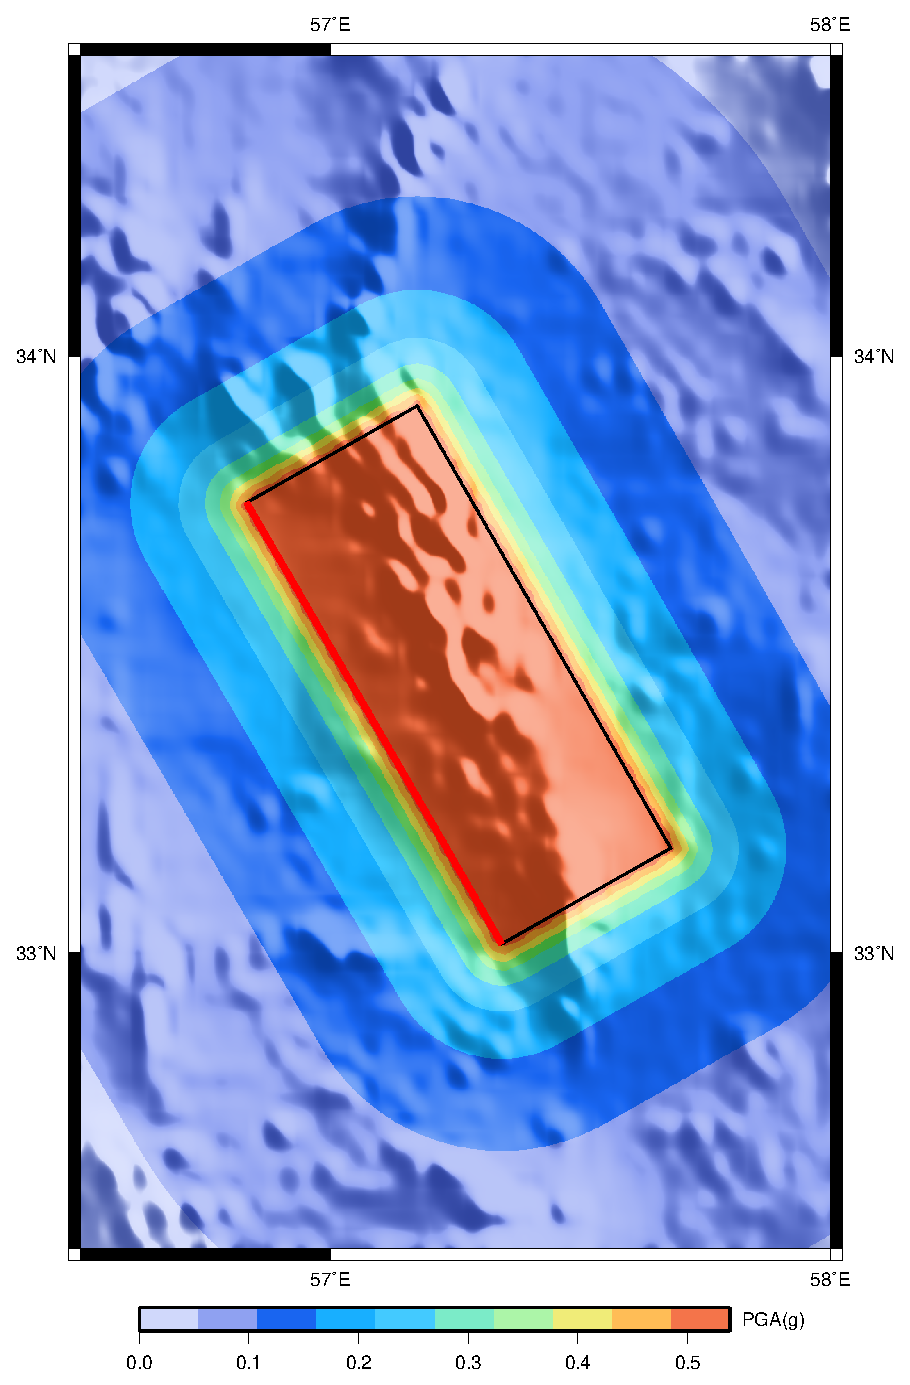
\includegraphics[width=5cm]{./Figures/Part_Hazard/medianGmfTabasPGA.eps}}
\subfigure[]{
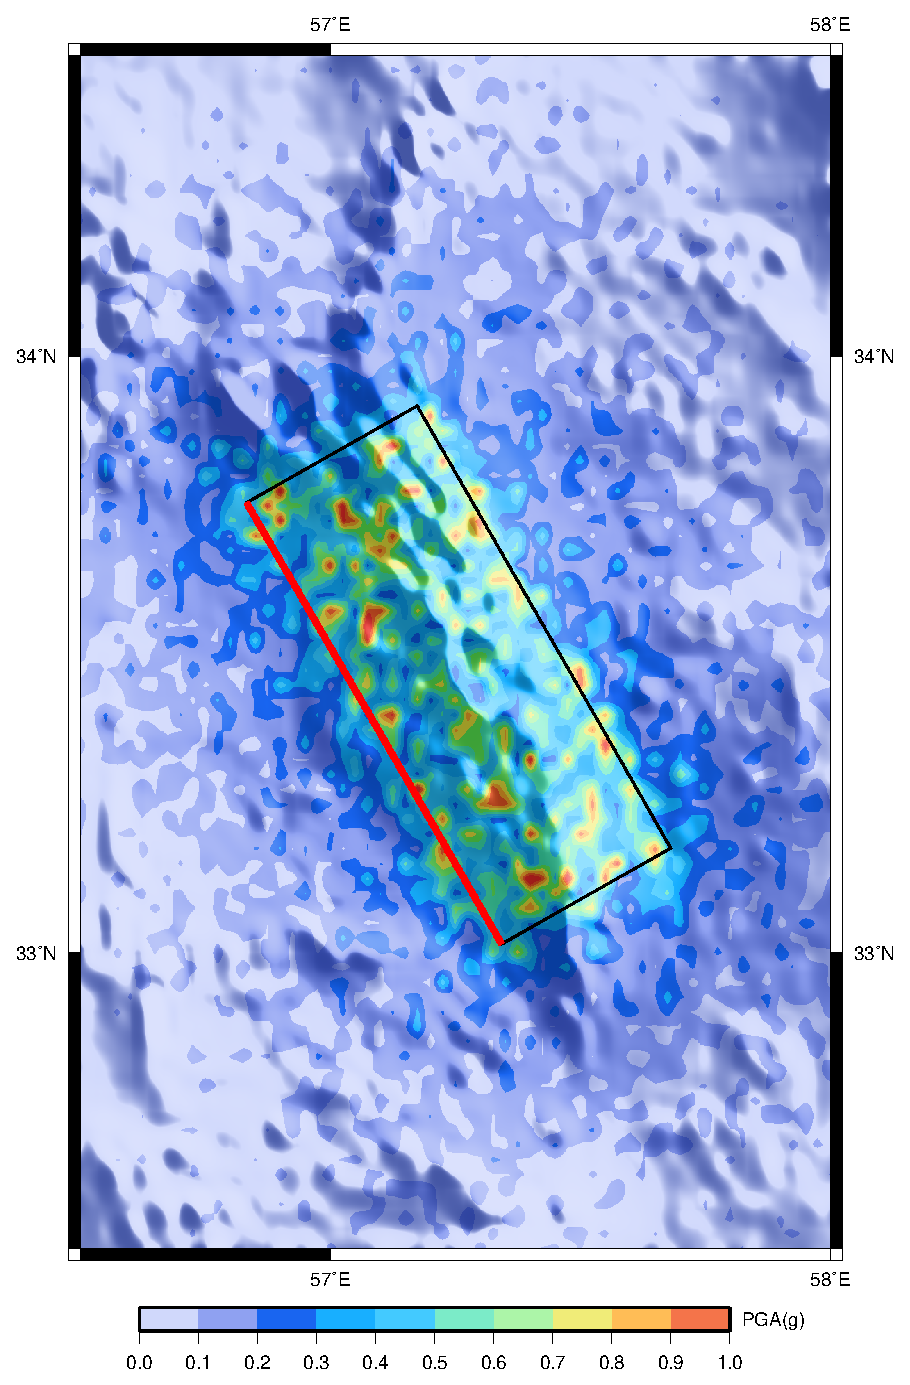
\includegraphics[width=5cm]{./Figures/Part_Hazard/uncorrelatedGmfTabasPGA.eps}}
\subfigure[]{
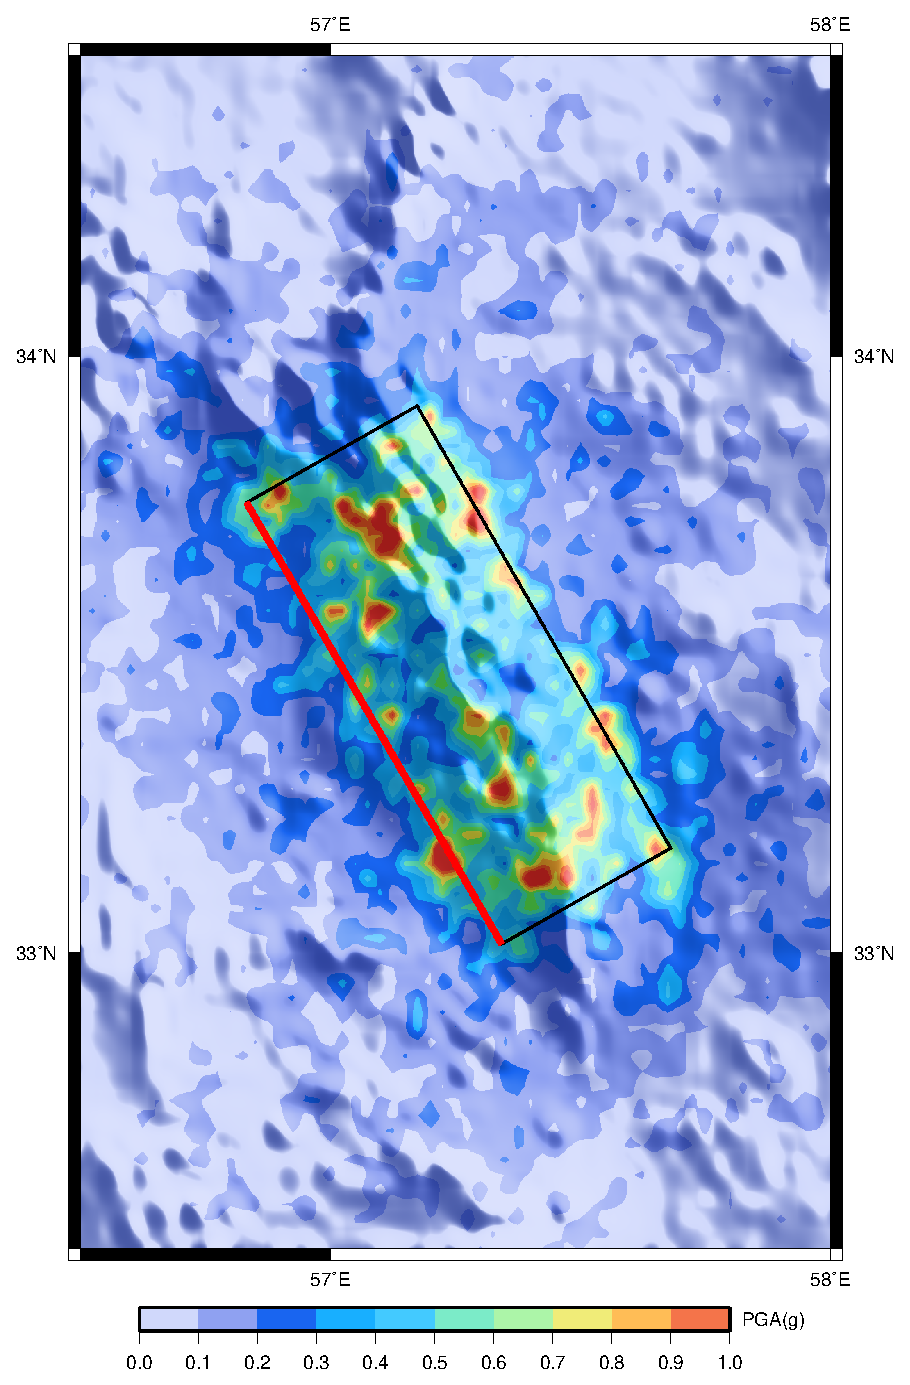
\includegraphics[width=5cm]{./Figures/Part_Hazard/correlatedGmfTabasPGA.eps}}
\subfigure[]{
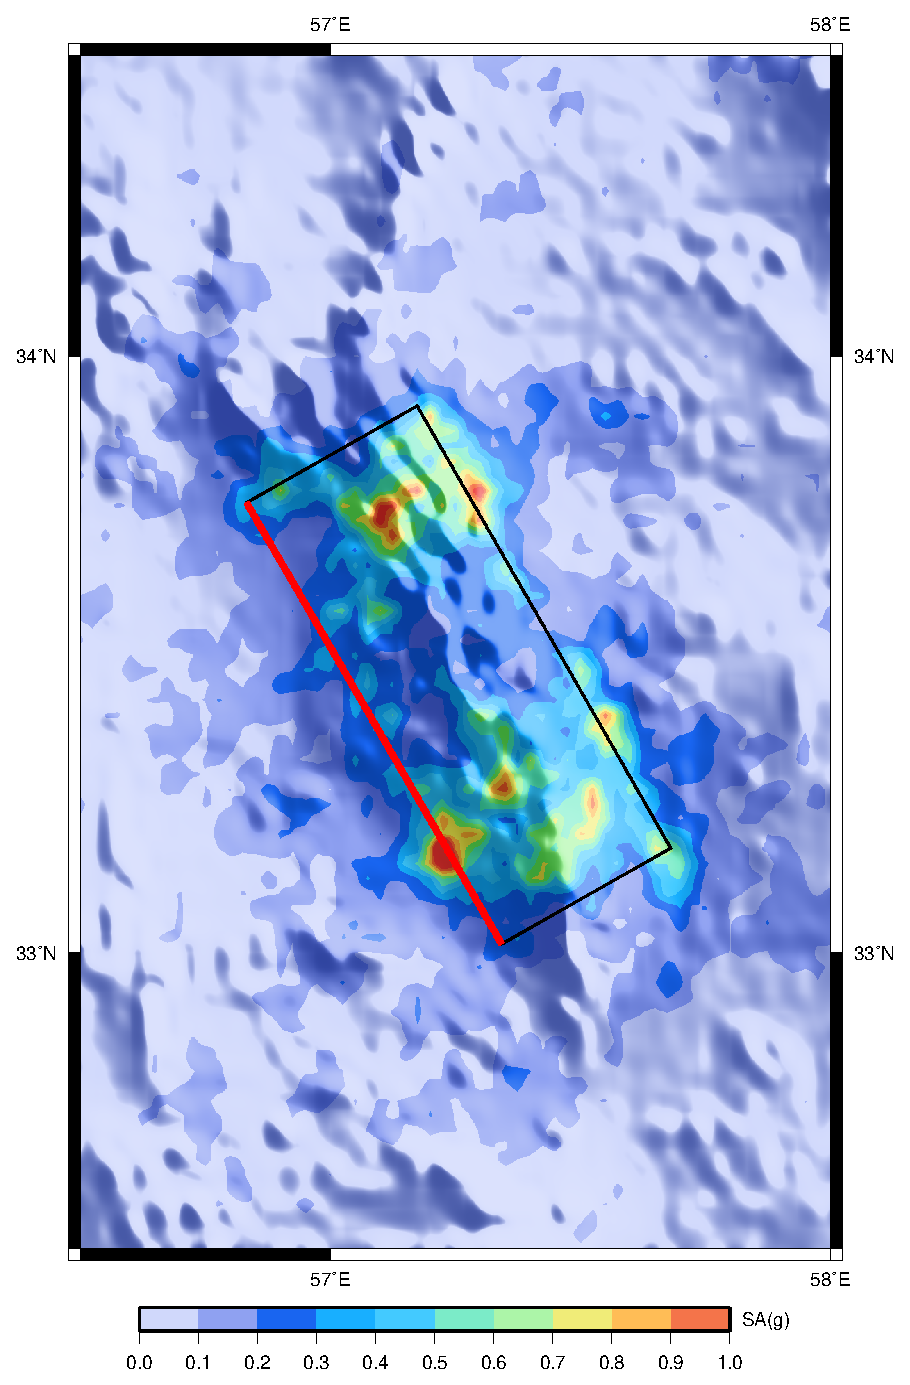
\includegraphics[width=5cm]{./Figures/Part_Hazard/correlatedGmfTabasSA.eps}}
\caption{Examples of median (a), intra-event uncorrelated (b), intra-event correlated for PGA (c) and for SA at $T=1$s (d). A rectangular planar rupture is considered as source of the shaking (the red line depicts the rupture trace, and the black line the rupture border). The rupture is associated to a magnitude 7 earthquake. The ground motion is estimated using the Boore and Atkinson 2008 GMPE (\cite{boore2008})}
\label{gmfs}
\end{center}
\end{figure}
%
%-------------------------------------------------------------------------------
\clearpage\newpage
\section{PSHA disaggregation}
\label{chap:disaggregation}
%
Seismic hazard disaggregation - or deaggregation - \citep{mcguire1995,bazzurro1999} is a procedure aimed at identifying the contributions to a specified level of hazard coming from different combinations
of basic variables - such as magnitude and rupture-site distance - characterizing the ruptures included in the ERF.
%
Two are the main typologies of disaggregation currently adopted in PSHA studies (see for example \citet{petersen2008}): the M-R-$\epsilon$ disaggregation and the geographic disaggregation. Conceptually there are no differences between the two; simply we can observe that in the geographic disaggregation the source-to-rupture distance is replaced by the position on the topographic surface of the rupture-point used to calculate the distance to the site.
%

\subsection{M-D disaggregation}
We start the description of the disaggregation procedure by considering the  simplest disaggregation case. 

As a first step we create a container where to progressively store the contributions coming from the different ruptures produced by the seismic sources contained in the Seismic Source Model.
%
To this purpose, we use a two-dimensional matrix $Q$ with a number or rows equal to the number of discrete distance bins and a number of columns equal to the number of discrete magnitude intervals. The magnitude and distance ranges used to create the $Q$ matrix cover the spectrum of values used in the hazard calculation. In particular, the magnitude range can be determined considering the properties of the seismicity occurrence model for each of the sources contained in the Seismic Source Model whilst the distance range is implicitly defined by a maximum integration distance parameter to be specified in the OQ configuration file. 
%

The argument of the summation contained in Equation \ref{eq:PSHA_calculation} computes the probability of exceedance in a time $t$ of $gm$ generated by the occurrence of the rupture $Rup$. Without loss of generality a rupture can be associated to a magnitude and a source-to-site distance.



